\section{Protocolo}
Toda a informação presente foi obtida da documentação do \textit{Signal} \cite{signal}.

\subsection{Primitivas}
Sem contar com os algoritmos referidos nas subsecções abaixo, que são uma grande parte do que torna o \textit{Signal} seguro, este também usa as primitivas, atualmente, mais seguras.

Algumas das primitivas e algoritmos que o \textit{Signal} utiliza são:
\begin{itemize}
    \item \textbf{\textit{SHA-512}}
    \begin{itemize}
        \item É uma função \textit{hash} criptográfica cuja operação mapeia dados de comprimento variável em dados de comprimento fixo, sendo os dados de comprimento fixo característicos do texto original e difíceis de reverter \footnote{difícil de encontrar duas mensagens com a mesma hash e difícil de  encontrar o texto original.}.
        \item Este algoritmo apresenta um número de combinações dado pela equação:
        \begin{equation}
            Combinacoes=2^{bits}=2^{512}=1.340781^{154}
        \end{equation}

        \item Isto implica que se alguém com um computador, imaginemos, a fazer $2^{16}$ cálculos em $\approx 0.2s$, isto é $327680$ cálculos por segundo, demoraria o seguinte intervalo de tempo a calcular todas essas combinações:
        \begin{equation}
            Tempo = 1.340781^{154} / 327680 = 4.091739^{148}s = 4.735809^{143} dias = 1.297482^{141} anos
        \end{equation}

        \item Colocando isto em perspetiva, sendo que a Terra tem $4,543\times10^9$ anos, um típico computador demoraria $1500 "Terras"$ a obter o total de combinações necessárias, isto é, seria necessário $1500$ vezes o tempo que a Terra existe para poder decifrar uma \textit{hash} efetuada com este algoritmo:
        \begin{equation}
        Tempo = 1.297482^{141} /4,543*10^{9} = 1.5740434^{18} ~= 1500 Terras
        \end{equation}
    \end{itemize}

    \item \textit{\textbf{Curve25519}}
    \begin{itemize}
        \item É uma curva elíptica que garante $128 bits$ de segurança, com \textit{elliptic curve Diffie-hellman key agreement}. Este foi construído de forma a evitar potenciais \textit{pitfalls} e para ser imune a \textit{time attacks} \footnote{ataques com base na análise do tempo gasto para executar algoritmos criptográficos.}.
    \end{itemize}

    \item \textit{\textbf{VXEdDSA}}
    \begin{itemize}
        \item É um algoritmo de \textit{signing} que usa a hash \textit{SHA-512}. Este funciona da seguinte forma:
        \begin{itemize}
            \item Sendo \textbf{k} uma chave privada Montgomery, \textbf{M} uma mensagem a ser assinada, \textbf{Z} uma sequência de 64 bytes aleatórios e seguros, \textbf{u} a chave pública Montgomery, \textbf{V||h||s} a assinatura a verificar(sequência de bytes em que \textbf{V} faz \textit{encode} de um ponto e \textbf{h} e \textbf{s} fazem \textit{encode} do \textit{integer modulo q(prime number)}), então temos os algoritmos dados pelo pseudocódigo em \ref{vxeddsa_sign} e \ref{vxeddsa_verify}:
            
            \begin{lstlisting}[caption=Assinatura de um documento,captionpos=b, label={vxeddsa_sign}]
                vxeddsa_sign(k, M, Z):
                    A, a = calculate_key_pair(k)
                    Bv = hash_to_point(A || M)
                    V = aBv
                    r = hash3(a || V || Z) (mod q)
                    R = rB
                    Rv = rBv
                    h = hash4(A || V || R || Rv || M) (mod q)
                    s = r + ha (mod q)
                    v = hash5(cV) (mod 2b)
                    return (V || h || s), v
                \end{lstlisting}
            
            \begin{lstlisting}[caption=Validação de assinatura de um documento,captionpos=b, label={vxeddsa_verify}]
                vxeddsa_verify(u, M, (V || h || s)):
                    if u >= p or V.y >= 2|p| or h >= 2|q| or s >= 2|q|:
                        return false
                    A = convert_mont(u)
                    Bv = hash_to_point(A || M)
                    if not on_curve(A) or not on_curve(V):
                        return false
                    if cA == I or cV == I or Bv == I:
                        return false
                    R = sB - hA
                    Rv = sBv - hV
                    hcheck = hash4(A || V || R || Rv || M) (mod q)
                    if bytes_equal(h, hcheck):
                        v = hash5(cV) (mod 2b)
                        return v
                    return false
            \end{lstlisting}
        \end{itemize}
    \end{itemize}
\end{itemize}

\subsection{KDF chains}\label{sec:KDF}
\textit{KDF Chains} faz parte do \emph{core} de um dos principais métodos, \emph{Double Ratchet} (secção \ref{sec:DoubleRatchet}), necessários para manter o \textbf{\textit{Signal}} seguro.
Este algoritmo recebe um \textbf{segredo}, uma \textbf{chave aleatória \textit{KDF}} e dados de \emph{input} e retorna um \emph{output} indistinguível de um qualquer texto gerado aleatóriamente, isto se a chave não for conhecida.
O termo \emph{KDF Chain} é usado quando parte do \emph{output} de uma \emph{KDF} é usado para substituir a \textbf{chave aleatória \textit{KDF}}, podendo assim esta ser usada para outro \emph{input}. O diagrama \ref{diagram:kdfChain} representa o processo de 3 \emph{inputs} produzirem 3 novas \emph{output keys}.


\begin{figure}[H]
\begin{center}
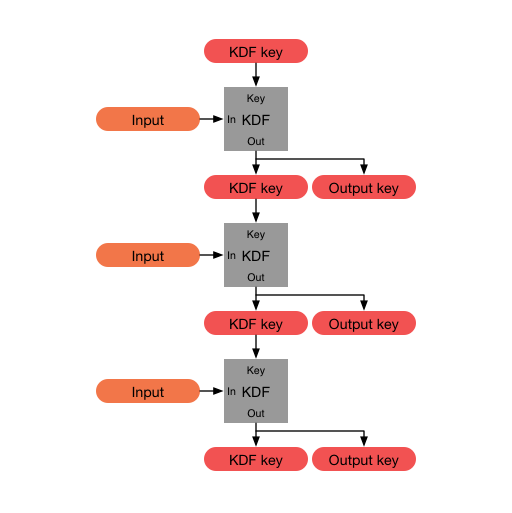
\includegraphics[width=12cm]{img/kdfChain.png}
\caption{KDF Chain com 3 inputs.}
\label{diagram:kdfChain}
\centering
\end{center}
\end{figure}

Uma \emph{KDF Chain} apresenta as seguintes propriedades:

\begin{itemize}
    \item \textbf{Resiliência}: se não houver conhecimento da chave \textit{KDF}, as chaves de output aparentam ser \emph{random}. Isto mantém-se verdadeiro mesmo que o atacante controle parte dos \emph{inputs}.
    \item \textbf{\textit{Forward Security}}: chaves de \textit{output} do passado aparentam ser \emph{random} para um atacante que conheceu uma chave \textit{KDF} num momento futuro.
    \item \textbf{\textit{Break-in recovery}}: se os inputs futuros adicionarem entropia suficiente, as chaves \textit{output} do futuro aparentam ser \emph{random} para um atacante que conheceu uma chave \textit{KDF} num momento qualquer.
\end{itemize}

Numa sessão que utilize \textbf{\textit{Double Ratchet}} (secção \ref{sec:DoubleRatchet}), imaginemos entre a Alice e o Bob, cada utilizador guarda 3 chaves, uma para cada \textit{KDF chain}: \textbf{\textit{root chain}}, \textbf{\textit{sending chain}} e \textbf{\textit{receiving chain}}. A chave \textit{sending} da Alice é equivalente à chave \textit{receiving} do Bob.

Por cada mensagem enviada e/ou recebida, a \emph{chain} "avança" e as suas chaves de \emph{output} são usadas para encriptar e/ou desencriptar as mensagens. A este processo dá-se o nome de \textbf{\textit{symmetric-key ratchet}}.


\subsection{Symmetric-key ratchet}\label{sec:symkey}

Todas e quaisquer mensagens enviadas ou recebidas são encriptadas usando uma \textbf{chave de mensagem única}. Esta chave única corresponde a uma chave de \textit{output} das \textit{KDF Chains} (secção \ref{sec:KDF}) correspondentes. Chamemos a estas chaves \textit{chain keys}.

Os \textit{inputs} na \textit{KDF Chain} para envio e receção são constantes, pelo que, por esta razão, não fornecem \textit{break-in recovery}. As suas \textit{chains} apenas garantem que cada mensagem é encriptada com uma chave única que pode ser eliminada após encriptação ou desencriptação. Calcular a próxima chave da \textit{chain} e de mensagem corresponde a um simples \textit{ratchet step} no algoritmo \textit{symmetric-key ratchet}.
O diagrama em baixo (diagrama \ref{diagram:skRatchet}) demonstra a execução deste algoritmo efetuando 2 \textit{ratchet steps}.

\begin{figure}[H]
\begin{center}
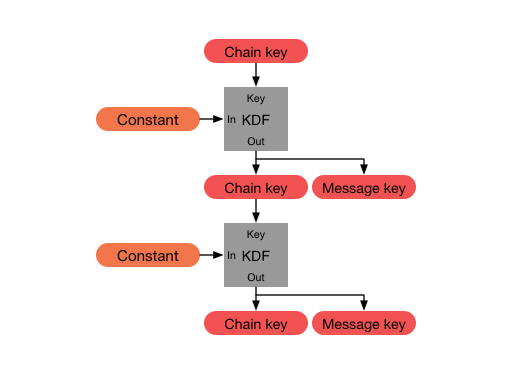
\includegraphics[width=12cm]{img/skRatchet.png}
\caption{Symmetric-key ratchet with 2 steps.}
\label{diagram:skRatchet}
\centering
\end{center}
\end{figure}

\subsection{Diffie-Hellman ratchet}\label{sec:dhratchet}
Até este momento, mencionamos \textit{KDF chains e Symmetric-key ratchet}, sendo estes algoritmos necessários para o funcionamento do \textit{Double Ratchet} (secção \ref{sec:DoubleRatchet}). No entanto, estes por si só não garantem que um atacante possuindo \textit{receiving chain keys} ou \textit{sending chain keys} não consiga gerar as futuras chaves e desencriptar todas as mensagens futuras. Para evitar isto, o \textit{Signal} combina \textit{symmetric-key ratchet} com \textit{DH Ratchet}.

Para implementar um \textit{Diffie-Hellman ratchet}, cada usuário gera um par de chaves \textit{Diffie-Hellman} (\textit{\textbf{ratchet key pair}}). Todas as mensagens trocadas entre estes 2 usuários vão ter no header a \textbf{chave pública}. Quando o receptor recebe a chave pública do emissor, é efetuado um \textbf{\textit{DH ratchet step}}, que consiste em substituir o actual \textbf{\textit{ratchet key pair}} por um novo par.

Este processo leva a que ambos usuários estejam constantemente a trocar as \textbf{\textit{ratchet key pair}}. Desta forma, se um dos usuários for comprometido, isto é, se um atacante obter a chave privada da \textit{ratchet}, apenas fica comprometida uma mensagem, e todas as mensagens anteriores e posteriores continuam seguras.

Os diagramas que se seguem, juntamente com o texto que os acompanham, demonstram mais especificamente o processo do \textbf{\textit{DH Ratchet}}:

\begin{enumerate}
    \item A Alice é "inicializada" com a \textit{ratchet key} pública do Bob. Desta forma, a chave pública da Alice ainda não é conhecida pelo Bob. A Alice executa um calculo \textit{Diffie-Hellman} entre a sua \textit{private ratchet key} e a \textit{public ratchet key} do Bob (figura \ref{diagram:DH1}).

    \begin{figure}[H]
        \begin{center}
            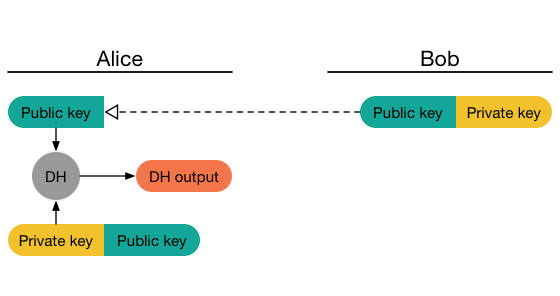
\includegraphics[width=12cm]{img/DH1.png}
            \caption{Mensagem enviada do Bob para a Alice.}
            \label{diagram:DH1}
        \end{center}
    \end{figure}

    \item A primeira mensagem enviada pela Alice anuncia a sua \textit{ratchet key} pública. Quando o Bob recebe uma destas mensagens, ele calcula um \textit{DH output} entre a \textit{ratchet key} pública da Alice e a sua \textit{ratchet key} privada, o que garante (através das propriedades do \textit{DH}) que, caso não tenha havido um \textit{middle-man}, seja igual ao \textit{output} inicial da Alice. O Bob, posteriormente, substitui o seu par de \textit{ratchet keys} e calcula um novo \textit{DH output} (figura \ref{diagram:DH2}).

    \begin{figure}[H]
        \begin{center}
            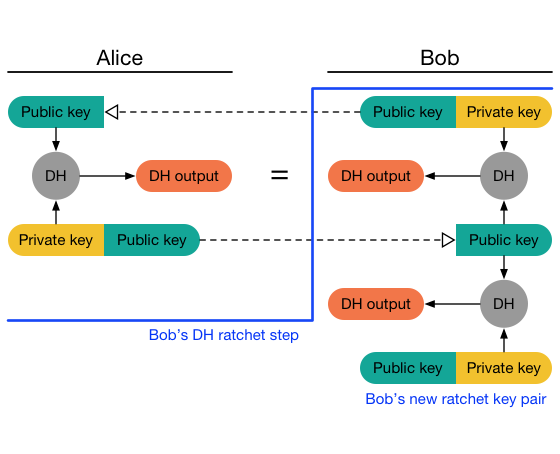
\includegraphics[width=12cm]{img/DH2.png}
            \caption{Mensagem enviada da Alice para o Bob após a mensagem inicial.}
            \label{diagram:DH2}
        \end{center}
    \end{figure}

    \item Uma nova mensagem vinda do Bob anuncia a sua nova \textit{ratchet key} pública. Quando a Alice recebe esta mensagem, vai executar um passo de \textit{DH ratchet}, substituindo o seu par de \textit{ratchet keys} e derivando 2 novos \textit{DH outputs}, um que será equivalente ao ultimo \textit{DH output} do Bob e um novo para ser usado na próxima mensagem (figura \ref{diagram:DH3}).

    \begin{figure}[H]
        \begin{center}
            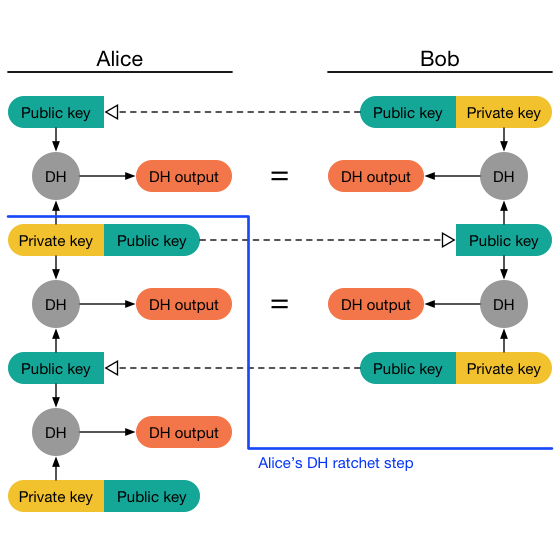
\includegraphics[width=12cm]{img/DH3.png}
            \caption{Nova mensagem do Bob, com a Alice como destinatário.}
            \label{diagram:DH3}
        \end{center}
    \end{figure}

    \item Uma mensagem nova por parte da Alice anuncia a sua nova chave pública. Eventualmente o Bob ira receber uma destas mensagens e executar um passo de \textit{DH ratchet} e assim sucessivamente (figura \ref{diagram:DH4}).

    \begin{figure}[H]
        \begin{center}
            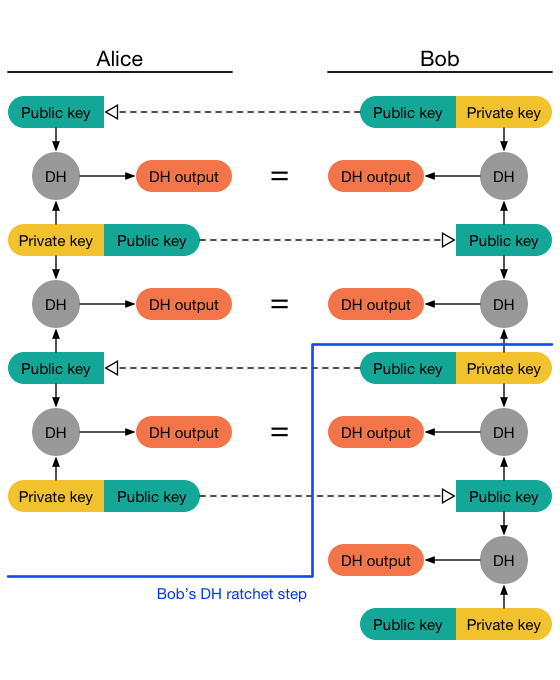
\includegraphics[width=12cm]{img/DH4.png}
            \label{diagram:DH4}
            \caption{Nova mensagem por parte da Alice.}
        \end{center}
    \end{figure}

    \item Os \textit{DH output} que são gerados em cada passo de \textit{DH ratchet} são usados para derivar novas chaves de envio e receção. A imagem abaixo (figura \ref{diagram:DH5}) revisita o primeiro passo do \textit{DH ratchet} efetuado pelo Bob. Nesta imagem o Bob usa o seu primeiro \textit{DH output} para derivar a sua chave de receção, que será equivalente à chave de envio por parte da Alice.

    \begin{figure}[H]
        \begin{center}
            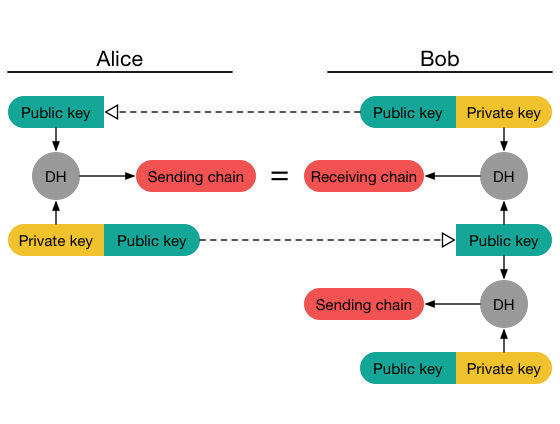
\includegraphics[width=12cm]{img/DH5.png}
            \caption{Mensagem inicial por parte do Bob e resposta por parte da Alice, mostrando mais       especificamente as cadeias de receção e de envio.}
            \label{diagram:DH5}
        \end{center}
    \end{figure}

    \item Sendo que os usuários efetuam "turnos" a executar um passo do \textit{DH Ratchet}, cada um toma turnos a introduzir novas cadeias de envio (figura \ref{diagram:DH6}).

    \begin{figure}[H]
        \begin{center}
            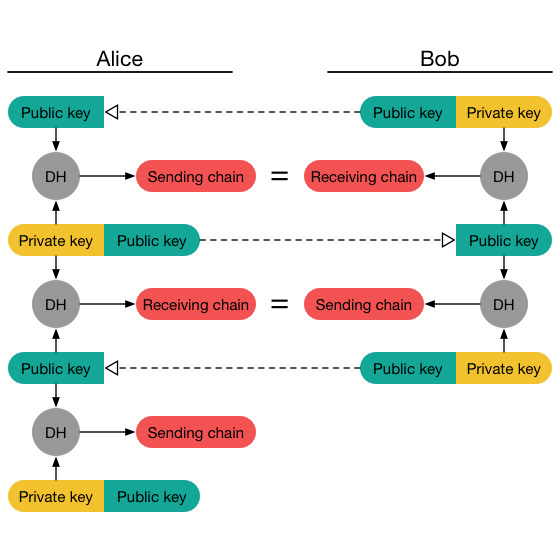
\includegraphics[width=12cm]{img/DH6.png}
            \caption{Nova mensagem por parte do Bob, mostrando as cadeias de receção e de envio.}
            \label{diagram:DH6}
        \end{center}
    \end{figure}

    \item No entanto, a imagem acima (figura \ref{diagram:DH6}), é uma simplificado. Em vez de se usar diretamente os \textit{DH outputs}, estes são usados como \textit{KDF (secção \ref{sec:KDF}) inputs} para uma \textit{root chain}, sendo os \textit{KDF outputs} da \textit{root chain} usados como chaves de envio e receção. Usar \textit{KDF} aumenta a resiliência e \textit{break-in recovery}.
    Desta forma ,um passo completo de uma \textit{DH Ratchet} consiste em atualizar a \textit{root KDF chain} $2\times$ e usar as \textit{DH output keys} como as novas chaves de envio e receção (figura \ref{diagram:DH7}).

    \begin{figure}[H]
        \begin{center}
            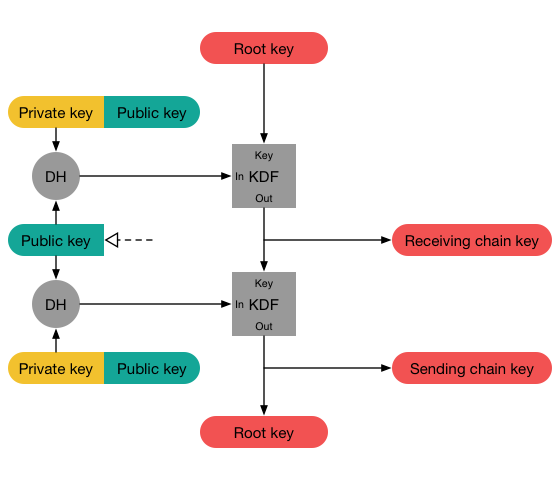
\includegraphics[width=12cm]{img/DH7.png}
            \caption{Imagem que demonstra o processo por de trás da geração das cadeias mencionadas nas imagens das figuras \ref{diagram:DH5} e \ref{diagram:DH6}.}
            \label{diagram:DH7}
        \end{center}
    \end{figure}
    
\end{enumerate}

\subsection{Double Ratchet}\label{sec:DoubleRatchet}
\subsubsection{Para que serve Double Ratchet?}
O algoritmo \emph{Double Ratchet} é um algoritmo usado por dois usuários (duma aplicação móvel, por exemplo) na troca de mensagens encriptadas baseadas numa chave secreta partilhada entre os dois. Ambos os usuários derivam uma nova chave por cada mensagem, de forma a que chaves anteriores não possam ser calculadas através da chaves mais recentes. Os usuários enviam valores públicos de \emph{Diffie-Hellman} juntamente com as suas mensagens. Os resultados dos cálculos de \emph{Diffie-Hellman} são misturados com a chave derivada anteriormente, de modo a que chaves anteriores não possam calcular chaves mais recentes. Estas propriedades garantem proteção perante das mensagens encriptadas caso exista o comprometimento das chaves de um dos usuários.

\subsubsection{Como funciona o Double Ratchet?}
A algoritmo de \textit{\textbf{Double Ratchet}} é a combinação de \textit{Symmetric-Key (secção \ref{sec:symkey})} com \textit{DH Ratchets (secção \ref{sec:dhratchet})} :

\begin{itemize}
    \item Quando uma mensagem é enviada ou recebida, um passo de \textit{Symmetric-Key ratchet} é aplicado nas cadeias de envio ou receção para derivar a nossa chave da mensagem.
    \item Quando uma nova chave \textit{ratchet public} é recebida, um passo de \textit{DH ratchet} é efetuado antes da \textit{symmetric-key ratchet} para substituir as chaves da cadeia (\textit{chain keys}).
\end{itemize}

No diagrama \ref{diagram:DR1}, em baixo, a Alice inicializou o processo com a chave \textit{ratchet public} e um segredo partilhado (equivalente à chave raiz inicial). Na inicialização a Alice gera um novo par de chaves \textit{ratchet} e envia o \textit{DH output} para a raiz do \textit{KDF}, de forma a que sejam calculadas uma nova chave raiz e uma nova chave de envio.

\begin{figure}[H]
    \begin{center}
        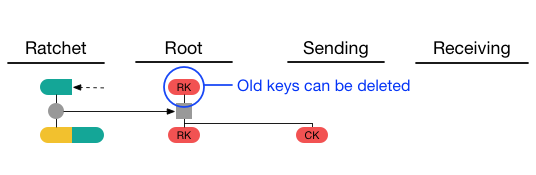
\includegraphics[width=12cm]{img/DR1.png}
        \caption{Primeira mensagem por parte do Bob e inicialização da chave raiz e chave de envio.}
        \label{diagram:DR1}
    \end{center}
\end{figure}

Quando a Alice envia a sua primeira mensagem, ela aplica um passo da \textit{symmetric-key ratchet} à sua cadeia de chaves de envio, resultando numa nova chave para as mensagens (cada chave deste género possuirá um \textit{label} perante a mensagem que estas encriptam/desencriptam). A nova chave da cadeia é guardada, enquanto que a chave para a mensagem e a antiga chave de cadeia podem ser eliminadas (figura \ref{diagram:DR2}).

\begin{figure}[H]
\begin{center}
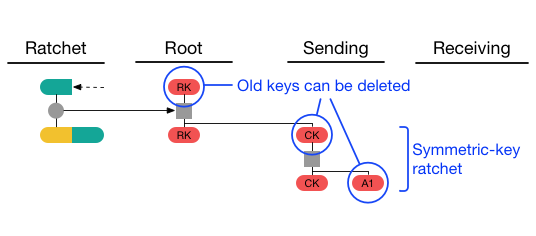
\includegraphics[width=12cm]{img/DR2.png}
\caption{Demonstração de um passo na \textit{symmetric-key ratchet} após receção da primeira mensagem.}
\label{diagram:DR2} 
\centering
\end{center}
\end{figure}

Se posteriormente a Alice receber uma mensagem vinda do Bob, esta irá conter uma nova chave \textit{ratchet public}. A Alice aplica um passo de \textit{DH ratchet} de forma a derivar novas chaves de envio e receção. Posteriormente, aplica um passo \textit{symmetric-key ratchet} na cadeia de receção para obter a chave de receção para a mensagem vinda do Bob (figura \ref{diagram:DR3}).

\begin{figure}[H]
\begin{center}
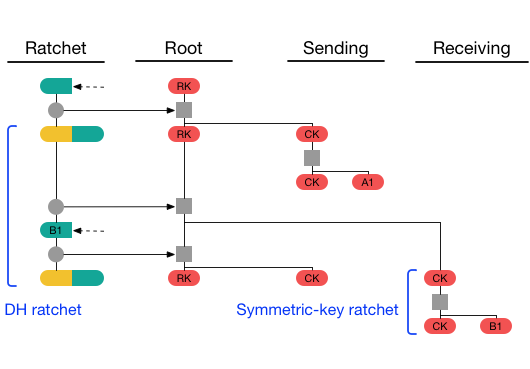
\includegraphics[width=12cm]{img/DR3.png}
\caption{Demonstração de um passo na \textit{symmetric-key ratchet} após receção da segunda mensagem vinda do Bob levando à geração de uma chave de receção.}
\label{diagram:DR3} 
\centering
\end{center}
\end{figure}

Suponhamos que a Alice envia uma mensagem A2, recebe uma mensagem B2 (com a chave \textit{ratchet public} antiga), depois envia a mensagem A3 e A4. A cadeia de envio da Alice faz 3 passos, enquanto a sua cadeia de receção apenas andou 1 passo (figura \ref{diagram:DR4}).

\begin{figure}[H]
\begin{center}
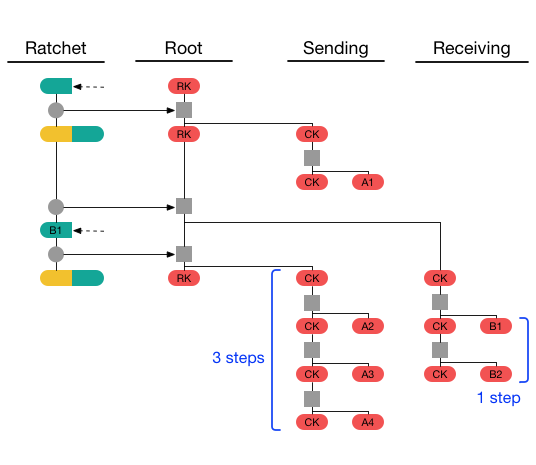
\includegraphics[width=12cm]{img/DR4.png}
\caption{Demonstração de alguns casos específicos do \textit{Double-Ratchet}.}
\label{diagram:DR4} 
\centering
\end{center}
\end{figure}

Se posteriormente receber a mensagem B3 e B4 com a próxima chave \textit{ratchet} do Bob e em seguida enviar a mensagem A5, o seu estado final será como o identificado no diagrama \ref{diagram:DR5}.

\begin{figure}[H]
\begin{center}
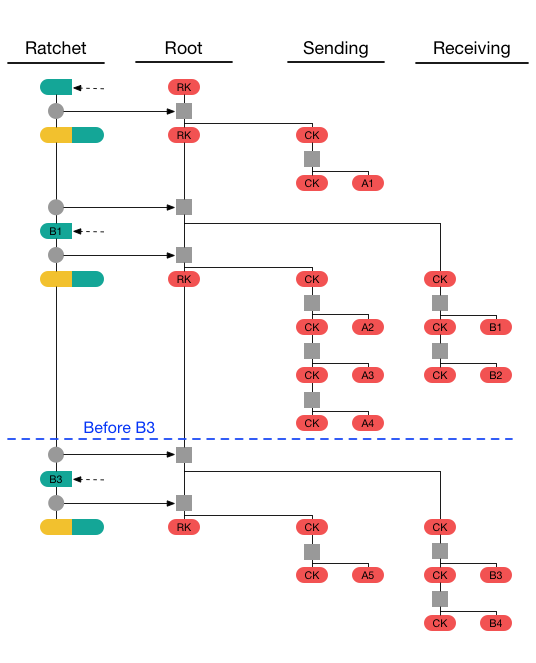
\includegraphics[width=12cm]{img/DR5.png}
\caption{Estado final da cadeia.}
\label{diagram:DR5} 
\centering
\end{center}
\end{figure}


\subsection{Será o protocolo do Signal realmente seguro?}

Perante tudo o que foi mencionado nos protocolos usados pelo \textit{Signal}, rapidamente poderíamos considerar que sim, o \textit{Signal} é bastante seguro. No entanto, sem qualquer acesso ao \textit{source-code}, não conseguimos validar realmente o quão solido e seguro ele é. Aqui entra uma das grandes razões para o \textit{Signal} ser o protocolo e aplicação mais segura de todas as existentes (sendo até usado por entidades políticas de grandes países \cite{politicsSignal}), pois ele é \textbf{\textit{open-Source}}, permitindo que qualquer pessoa analise o código fonte, detete erros no mesmo e os possa, inclusivé, corrigir. O protocolo utilizado tornou-se tão popular, seguro e bem recebido pela comunidade dedicada a \textit{cibersegurança}, que passou a ser um protocolo por si mesmo, tendo sido este adaptado, em 2018, por aplicações de grandes empresas, como o \textit{WhatsApp}, \textit{Facebook Messenger}, \textit{Skype} ou \textit{Google Allo}. Apesar disso, em alguns destes, o \textit{Signal protocol} não se encontra ativado por defeito.

Para além do que já foi mencionado, o \textit{Signal} proporciona ainda uma excelente documentação \cite{signal}, onde explica detalhadamente todo o processo por detrás do seu protocolo, permitindo que qualquer engenheiro ou entusiasta valide o protocolo sem necessitar de analisar o código, podendo detetar lacunas antes de olhar para o mesmo. Por outro lado, o \textit{Signal} tem passado por varias auditorias, sem qualquer registo de falhas a nível de segurança.

Algumas auditorias e estudos feitos ao \textit{Signal}:
\begin{itemize}
    \item 2017, julho, investigadores de \textit{Ruhr University Bochum} durante uma nova análise detetam uma falha puramente teórica, uma vez que esta, ao acontecer, seria automaticamente detetada, validando o protocolo como \textbf{seguro} \cite{rosler2018more}.
    
    \item 2016, outubro, investigadores de \textit{University of Oxford,Queensland University of Technology and McMaster University} publicam uma analise formal do protocolo, concluído que o protocolo era \textbf{criptograficamente seguro} \cite{cohn2017formal}.

    \item 2014, outubro, investigadores de \textit{Ruhr University Bochum} publicam uma análise do protocolo \textbf{validando a sua segurança} \cite{frosch2016secure}.
\end{itemize}


\subsection{Domain Fronting e \textit{Signal} App}
No geral, a sociedade procura ter privacidade. No entanto, por outro lado, existem organizações, muitas vezes com interesses politicos, que pretendem obter mais informação sobre a população ou dos cidadãos do seu pais. Desta forma, alguns países, como por exemplo o Egito, bloqueiam o tráfego de aplicações como o \textit{Signal}, tendo isso como consequência a redução da privacidade das pessoas \cite{noSignal}.

O \textit{Signal} tenta travar estas ações, mais uma vez procurando devolver a privacidade aos cidadãos, usando um mecanismo chamado \textbf{\textit{Domain Fronting}}. Este, como referido no artigo \cite{domainFrontingExplained}, funciona fazendo \textit{bypass} aos métodos de censura que o bloqueiam, através de \textit{DPI, DNS Filtering} e \textit{IP Blocking}, sendo que estes dependem de grandes \textit{CDN's}. Desta forma, o \textit{Domain Fronting} não passa de uma forma de fazer o tráfico parecer que é gerado por um \textit{domain} válido, isto é, não bloqueado no respetivo país. Isto apenas é possível pela forma como as \textit{CDN's} modernas funcionam, sendo que tudo acontece na \textit{application layer} da camada \textit{OSI} (figura \ref{diagram:OSI}). 

\begin{figure}[H]
    \begin{center}
        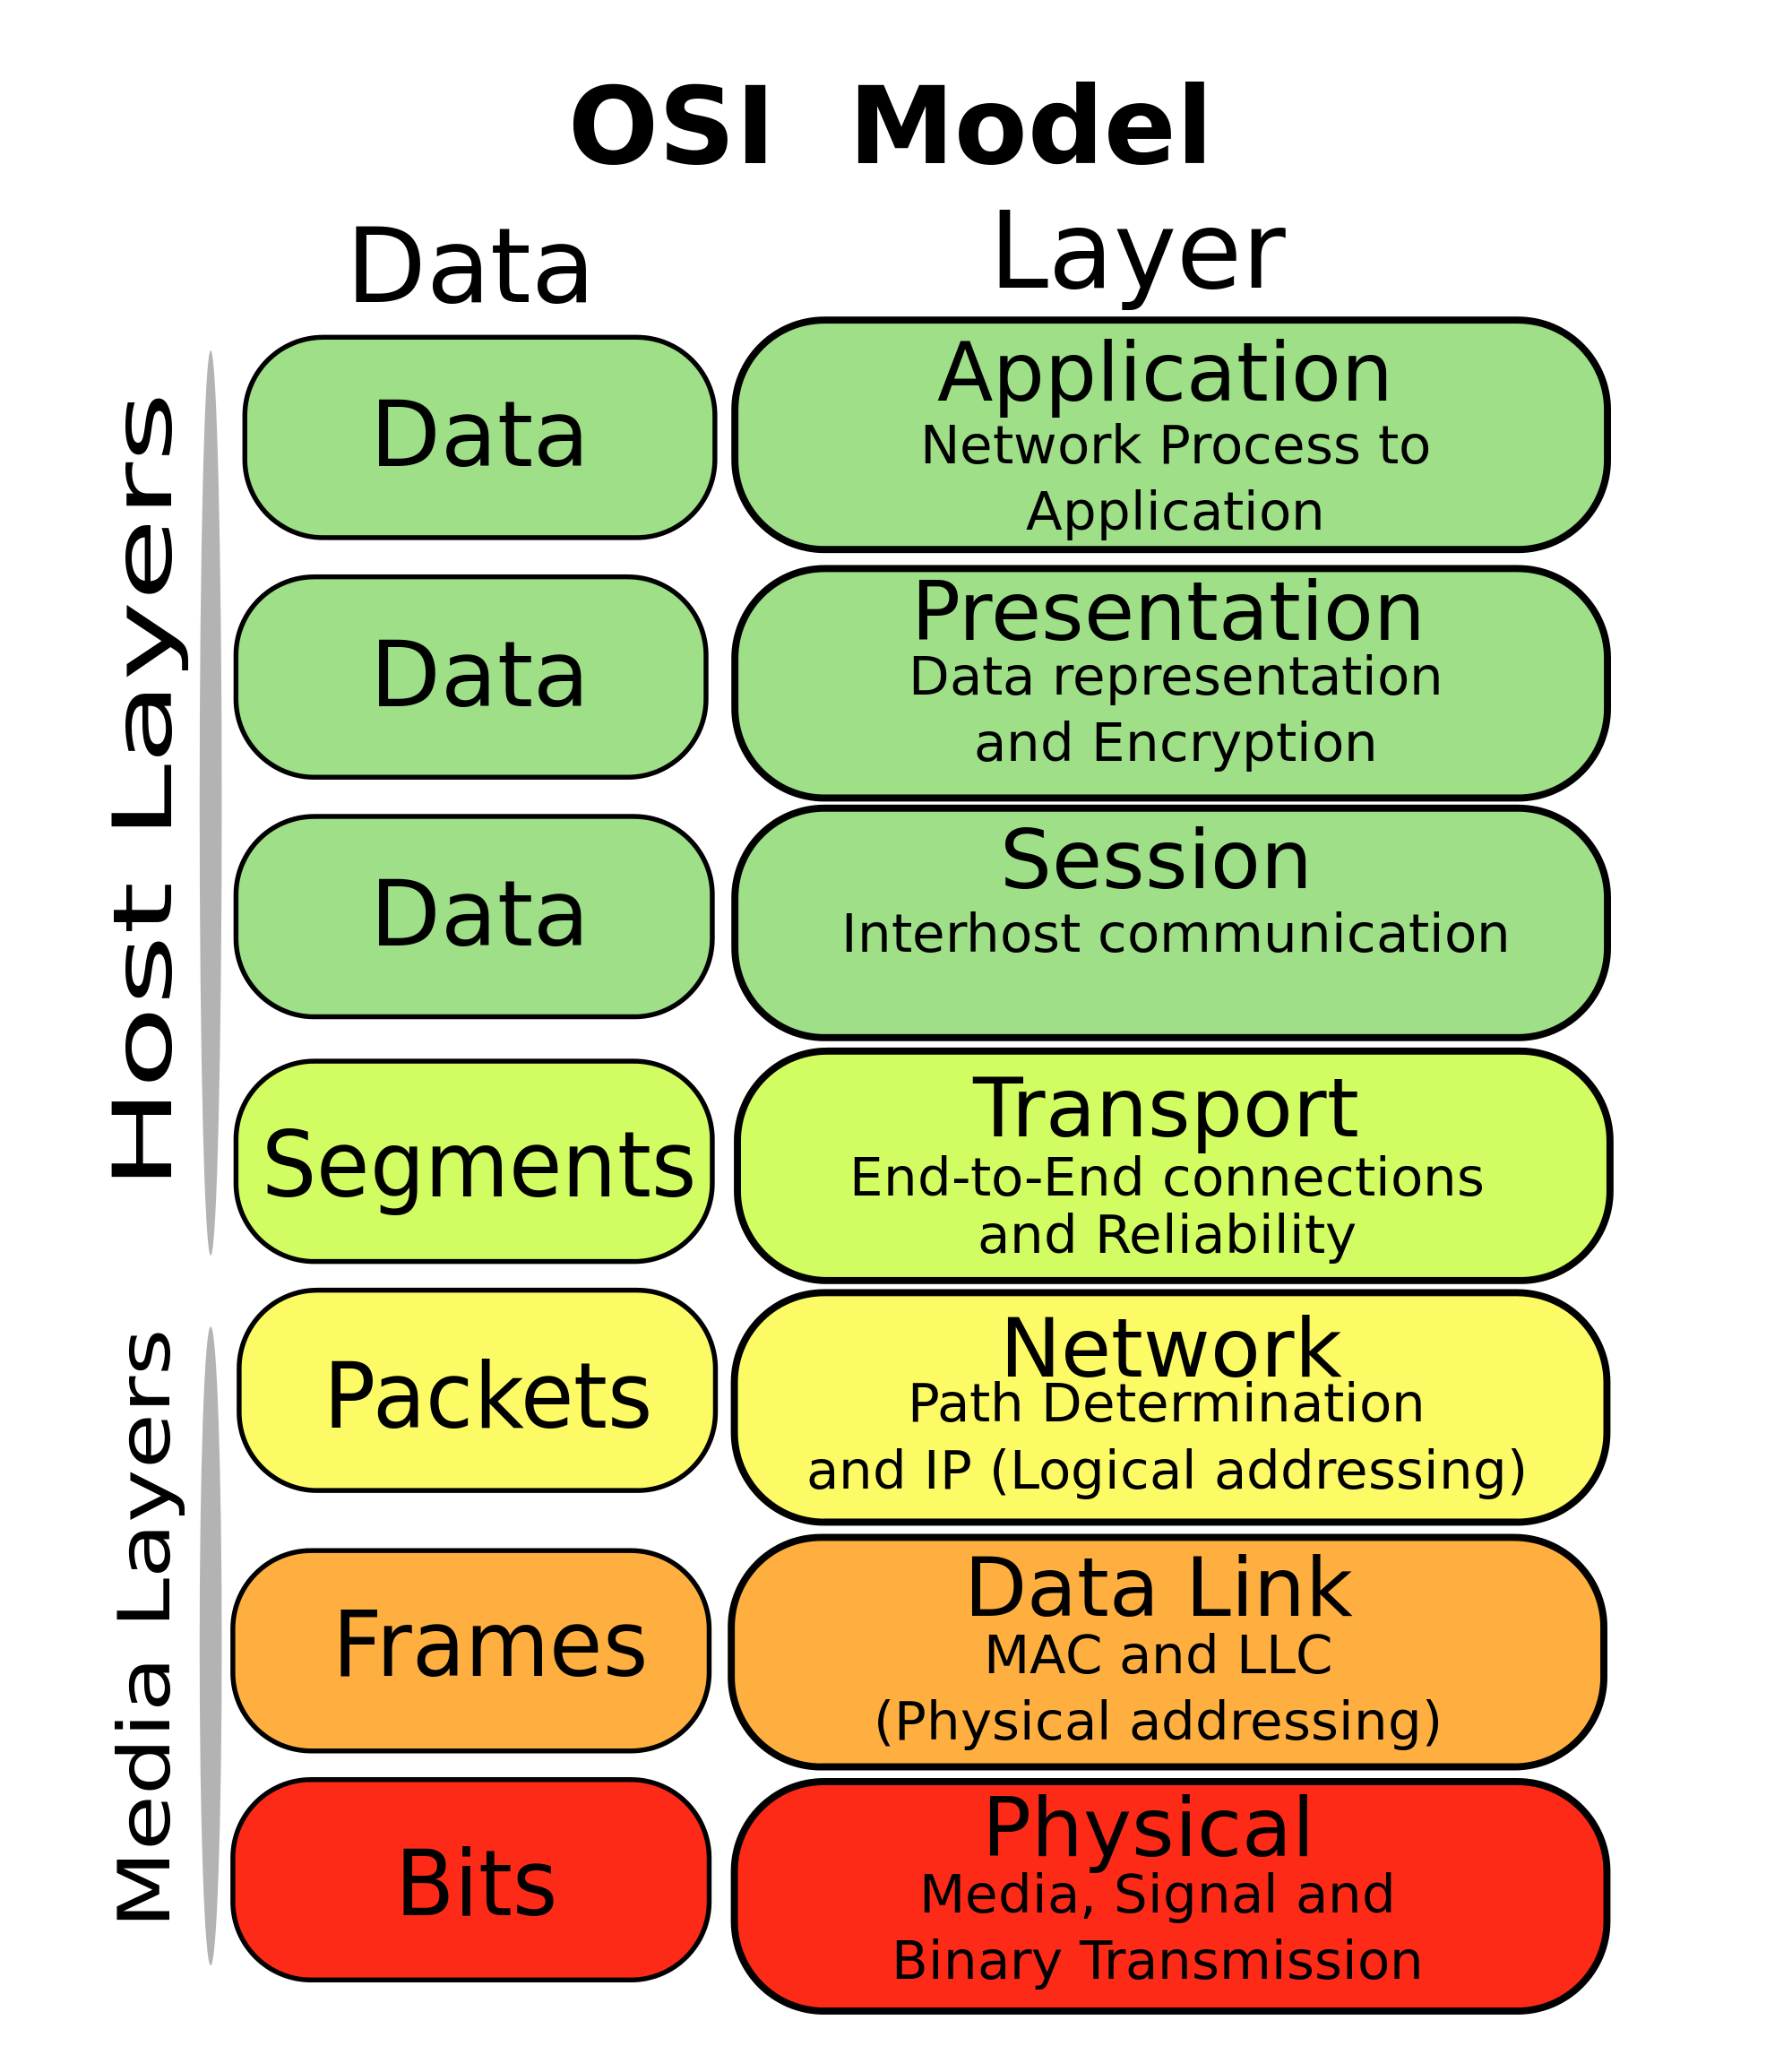
\includegraphics[width=12cm]{img/OSI.png}
        \caption{Representação das camadas \textit{OSI}, dando-se ênfase à camada aplicacional \cite{OSI}.}
        \label{diagram:OSI}
    \end{center}
\end{figure}

Por exemplo, imaginemos que o \textbf{\textit{Domain A}} e o \textbf{\textit{Domain B}} pertencem ao mesmo \textit{CDN}. No entanto, o \textbf{A} encontra-se bloqueado mas o \textbf{B} não. Assim, a ideia principal do \textit{Domain Fronting} é criar um pacote com o \textbf{\textit{Domain B}} no \textit{SNI Header} e o \textbf{\textit{Domain A}} no \textit{HTTP Header}. Uma vez que o \textit{SNI} não é encriptado no \textit{TLS Protocol}, este não será bloqueado pelas autoridades, mas quando o pedido chega ao CDN e lê o \textit{HTTP Host Header} com o \textbf{\textit{Domain A}}, a mensagem será encaminha para o \textbf{\textit{Domain A}} (fig. \ref{diagram:domainFronting}).

\begin{figure}[H]
    \begin{center}
        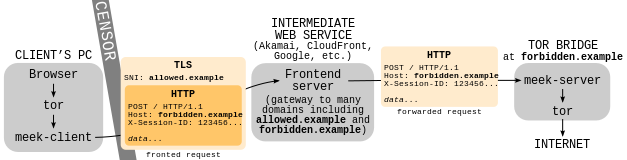
\includegraphics[width=15cm]{img/domainFronting.png}
        \caption{Funcionamento do Domain Fronting \cite{df}.}
        \label{diagram:domainFronting}
    \end{center}
\end{figure}


Como podemos perceber, o \textit{Signal} tenta sempre possibilitar e manter a privacidade dos seus usuários. No entanto, este método deixa de funcionar se, como mencionado no artigo do \textit{Signal} \cite{signalDomainFronting}, forem bloqueados todos os sites de um \textit{CDN} especifico para se bloquear o site que se pretende censurar (por exemplo, houve uma tentativa da Russia a bloquear o \textit{Telegram}, bloqueando todo o tráfego de uma \textit{CDN} \cite{domainFrontingExplained, domainFrontingBlock}). No final de contas, o \textit{Signal} perdeu o seu alcance nos países em que foi censurado, pois as \textit{CDN's} usadas bloquearam este tipo de comportamento (e.g Amazon Services bloqueia \textit{Signal} \cite{signalDomainFronting}), mas deixou uma marca que demonstra que, internamente, o seu protocolo visa e procura manter a privacidade das pessoas. Esta questão será melhor analisada na secção dos problemas associados a este serviço.
